% Options for packages loaded elsewhere
\PassOptionsToPackage{unicode}{hyperref}
\PassOptionsToPackage{hyphens}{url}
%
\documentclass[
  ignorenonframetext,
  aspectratio=169,
]{beamer}
\usepackage{pgfpages}
\setbeamertemplate{caption}[numbered]
\setbeamertemplate{caption label separator}{: }
\setbeamertemplate{navigation symbols}{}
\setbeamertemplate{footline}[page number]
\setbeamertemplate{itemize item}{\small\raise0.5pt\hbox{$\bullet$}}
\setbeamertemplate{itemize subitem}{\tiny\raise1.5pt\hbox{$\bullet$}}
\setbeamertemplate{itemize subsubitem}{\tiny\raise1.5pt\hbox{$\bullet$}}
\setbeamercolor{caption name}{fg=normal text.fg}
\beamertemplatenavigationsymbolsempty
% Prevent slide breaks in the middle of a paragraph
\widowpenalties 1 10000
\raggedbottom
\setbeamertemplate{part page}{
  \centering
  \begin{beamercolorbox}[sep=16pt,center]{part title}
    \usebeamerfont{part title}\insertpart\par
  \end{beamercolorbox}
}
\setbeamertemplate{section page}{
  \centering
  \begin{beamercolorbox}[sep=12pt,center]{part title}
    \usebeamerfont{section title}\insertsection\par
  \end{beamercolorbox}
}
\setbeamertemplate{subsection page}{
  \centering
  \begin{beamercolorbox}[sep=8pt,center]{part title}
    \usebeamerfont{subsection title}\insertsubsection\par
  \end{beamercolorbox}
}
\AtBeginPart{
  \frame{\partpage}
}
\AtBeginSection{
  \ifbibliography
  \else
    \frame{\sectionpage}
  \fi
}
\AtBeginSubsection{
  \frame{\subsectionpage}
}
\usepackage{amsmath,amssymb}
\usepackage{lmodern}
\usepackage{iftex}
\ifPDFTeX
  \usepackage[T1]{fontenc}
  \usepackage[utf8]{inputenc}
  \usepackage{textcomp} % provide euro and other symbols
\else % if luatex or xetex
  \ifXeTeX
    \usepackage{xltxtra} 
    \usepackage{xeCJK}
    \setCJKmainfont{ipaexm.ttf}
    \setCJKsansfont{ipaexg.ttf}
    \setCJKmonofont{ipaexg.ttf}
  \fi
  \usepackage{unicode-math}
  \defaultfontfeatures{Scale=MatchLowercase}
  \defaultfontfeatures[\rmfamily]{Ligatures=TeX,Scale=1}
\fi
% Use upquote if available, for straight quotes in verbatim environments
\IfFileExists{upquote.sty}{\usepackage{upquote}}{}
\IfFileExists{microtype.sty}{% use microtype if available
  \usepackage[]{microtype}
  \UseMicrotypeSet[protrusion]{basicmath} % disable protrusion for tt fonts
}{}
\makeatletter
\@ifundefined{KOMAClassName}{% if non-KOMA class
  \IfFileExists{parskip.sty}{%
    \usepackage{parskip}
  }{% else
    \setlength{\parindent}{0pt}
    \setlength{\parskip}{6pt plus 2pt minus 1pt}}
}{% if KOMA class
  \KOMAoptions{parskip=half}}
\makeatother
\usepackage{xcolor}
\IfFileExists{xurl.sty}{\usepackage{xurl}}{} % add URL line breaks if available
\IfFileExists{bookmark.sty}{\usepackage{bookmark}}{\usepackage{hyperref}}
\hypersetup{
  pdftitle={Estimating Effect of Tax Incentives on Charitable Giving Considering Self-Selection of Tax Relief in South Korea},
  hidelinks,
  pdfcreator={LaTeX via pandoc}}
\urlstyle{same} % disable monospaced font for URLs

\usepackage{setspace}
\usepackage{float}

\newif\ifbibliography
\usepackage{longtable,booktabs,array}
\usepackage{threeparttable, threeparttablex, multirow}
\usepackage{calc} % for calculating minipage widths
\usepackage{caption}
% Make caption package work with longtable
\makeatletter
\def\fnum@table{\tablename~\thetable}
\makeatother
\usepackage{graphicx}
\makeatletter
\def\maxwidth{\ifdim\Gin@nat@width>\linewidth\linewidth\else\Gin@nat@width\fi}
\def\maxheight{\ifdim\Gin@nat@height>\textheight\textheight\else\Gin@nat@height\fi}
\makeatother
% Scale images if necessary, so that they will not overflow the page
% margins by default, and it is still possible to overwrite the defaults
% using explicit options in \includegraphics[width, height, ...]{}
\setkeys{Gin}{width=\maxwidth,height=\maxheight,keepaspectratio}
% Set default figure placement to htbp
\makeatletter
\def\fps@figure{htbp}
\makeatother
\setlength{\emergencystretch}{3em} % prevent overfull lines
\providecommand{\tightlist}{%
  \setlength{\itemsep}{0pt}\setlength{\parskip}{0pt}}
\setcounter{secnumdepth}{-\maxdimen} % remove section numbering


\usepackage{siunitx}
\ifLuaTeX
  \usepackage{selnolig}  % disable illegal ligatures
\fi

\title{Estimating Effect of Tax Incentives on Charitable Giving Considering Self-Selection of Tax Relief in South Korea  }
\author[shortname]{ Hiroki Kato \inst{1} \and  Tsuyoshi Goto \inst{2} \and  Yong-Rok Kim \inst{3} \and }
\institute[shortinst]{ \inst{1} Osaka University \and  \inst{2} Chiba University \and  \inst{3} Kansai University \and }

\date{2022/04/19}


\begin{document}
\frame{\titlepage}

\begin{frame}{Tax Incentives on Donations}
\protect\hypertarget{tax-incentives-on-donations}{}
\begin{itemize}
\tightlist
\item
  Governments set a tax relief for charitable giving

  \begin{itemize}
  \tightlist
  \item
    if subsidizing charitable giving induces a large increase in donations, it is desirable for public good provision.
  \end{itemize}
\item
  Key parameter to evaluate social welfare: the price elasticity of charitable donations (Saez, 2004)

  \begin{itemize}
  \tightlist
  \item
    giving price: relative price to the private consumption
  \end{itemize}
\end{itemize}
\end{frame}

\begin{frame}{Literatures: Price Elasticity of Giving}
\protect\hypertarget{literatures-price-elasticity-of-giving}{}
\begin{itemize}
\tightlist
\item
  Large empirical literatures examining the giving price elasticity estimate log-log demand function to derive the giving price elasticity
\item
  Two types of data

  \begin{enumerate}
  \tightlist
  \item
    tax filing data: Randolph, 1995; Auten et al., 2002; Fack and Landais, 2010; Bakija and Heim, 2011; Almunia et al., 2020
  \item
    panel survey data: Rehavi and Shack, 2013; Yoruk, 2013; Zampelli and Yen, 2016; Backus and Grant, 2019
  \end{enumerate}
\item
  Issue: Although many of these papers consider the endogeneity issue such as the endogenous change of the marginal tax rate by the amount of giving, they pay less attention to the problems caused by the fact that \color{red}{tax payers have to declare their charitable giving to receive tax relief on charitable giving}.
\end{itemize}
\end{frame}

\begin{frame}{Literatures: Tax Compliance}
\protect\hypertarget{literatures-tax-compliance}{}
\begin{itemize}
\tightlist
\item
  Existence of compliance costs to apply measures of tax relives because everyone will apply the measures if there is no compliance cost.

  \begin{itemize}
  \tightlist
  \item
    tax payers apply the measures of tax relives only if their benefits from the measures exceed the compliance costs.
  \end{itemize}
\item
  Recent papers insist this point and suggest that the measures of tax relives may not work as the policy makers expected
\item
  They also suggest compliance costs (e.g.~record-keeping cost and a fee for accountants) are considerably high.

  \begin{itemize}
  \tightlist
  \item
    individual income tax (Benzarti, 2020); corporate income tax (Zwick, 2021); charitable giving (Fack and Landais, 2016;Gillitzer and Skov, 2018; Almunia et al., 2020)
  \end{itemize}
\end{itemize}
\end{frame}

\begin{frame}{What Our Paper Did}
\protect\hypertarget{what-our-paper-did}{}
\begin{itemize}
\tightlist
\item
  We bridge price elasticity of giving and self-selection of tax incentive

  \begin{itemize}
  \tightlist
  \item
    As long as we know, there is no paper in the literature of giving price elasticity consider the self selection problem
  \end{itemize}
\item
  We estimate the giving price elasticity using the South Korean (Korea, hereafter) survey panel data called the National Survey of Tax and Benefit (NaSTaB)
\item
  Why South Korea?

  \begin{enumerate}
  \tightlist
  \item
    Compliance costs for wage earners and self-employed workers are different (IV)
  \item
    We could consider the sample of low-income households, which are sometimes omitted from the tax filer data.
  \item
    We can exploit the South Korean tax reform in 2014 as a main identification strategy of price change (income deduction \(\to\) tax credit)
  \end{enumerate}
\end{itemize}
\end{frame}

\begin{frame}{What Our Paper Found}
\protect\hypertarget{what-our-paper-found}{}
Using the IV representing the compliance cost,

\begin{enumerate}
\tightlist
\item
  Intensive-margin price elasticities are in the range between \(XXX\) and \(XXX\)

  \begin{itemize}
  \tightlist
  \item
    FE model w/o IV: \(XXX\) (similar value to the estimates in the existing literature)
  \end{itemize}
\item
  Extensive-margin price elasticities are in the range between \(YYY\) and \(YYY\)

  \begin{itemize}
  \tightlist
  \item
    FE model w/o IV: \(YYY\)
  \end{itemize}
\end{enumerate}

We examine well-known issues in the robustness check

\begin{itemize}
\tightlist
\item
  intensive-margin tax-price elasticities are in the range of -2 and -1.5
\item
  extensive-margin tax-price elasticities are in the range of -5 and -1.7
\end{itemize}
\end{frame}

\hypertarget{background}{%
\section{Institutional background and Sources of Endogeneity}\label{background}}

\begin{frame}{Framework}
\protect\hypertarget{framework}{}
Consider that a household with pre-tax income \(y_i\) has a choice between private consumption \(x_i\) and charitable giving \(g_i\).

Their budget constraint can be shown as
\begin{align}
x_i + g_i = y_i - R_iK_i - R_iT(y_i, g_i) - (1-R_i)T(y_i). \label{eq:budget}
\end{align}

\begin{itemize}
\tightlist
\item
  \(T\) is tax amount which depends on the pre-tax income and charitable giving. Assume \(T_y(\cdot)>0\) and \(T_{yy}(\cdot)>0\).
\item
  \(R_i\) is the dummy which takes 1 if \(i\) declares the tax relief and 0 otherwise.
\item
  \(K_i\) is a fixed compliance cost for the declaration of charitable giving.

  \begin{itemize}
  \tightlist
  \item
    In the literature about the giving price elasticity, most of papers implicitly assume \(R_i=1\) and \(K_i=0\).
  \end{itemize}
\end{itemize}
\end{frame}

\begin{frame}{Decision Rule of Tax Relief}
\protect\hypertarget{decision-rule-of-tax-relief}{}
\begin{align}
  R_i = \begin{cases}
      1 \text{ if }T(y_i, g_i) + K_i<T(y_i)\\
      0 \text{ if }T(y_i, g_i) + K_i\ge T(y_i). \label{eq:R}
  \end{cases}
\end{align}

where

\begin{align}
  T(y_i, g_i) =
  \begin{cases} 
      T(y_i-g_i)&\text{ if tax relief is applied by income deduction.}\\
      T(y_i)-mg_i &\text{ if tax relief is applied by tax credit.} \label{eq:relief}
  \end{cases}
\end{align}
\end{frame}

\begin{frame}{Giving Price}
\protect\hypertarget{giving-price}{}
Let us differentiate the budget constraint \eqref{eq:budget} by \(x_i\) and \(g_i\).
Then, it derives that the giving price (relative to the private consumption) is
\(\frac{dx_i}{dg_i}=1+R_iT_g(y_i,g_i)\), which we denote \(p\).

\begin{align}
    p=
    \begin{cases} 
        1-R_iT'(y_i-g_i)&\text{ if tax relief is applied by income deduction.}\\
        1-R_im&\text{ if tax relief is applied by tax credit.}\label{giving price}
    \end{cases}
\end{align}
Hereafter,
let us \(q\) to show the amount of tax relief for each declared giving
(i.e.~\(p=1-R_iq\) and \(q=-T_g(y_i, g_i)\)).
The government can change \(q\) by the tax reform.
\end{frame}

\begin{frame}{Marginal Tax Rate}
\protect\hypertarget{marginal-tax-rate}{}
\begin{table}

\caption{\label{tab:mtr}Marginal Income Tax Rate}
\centering
\fontsize{9}{11}\selectfont
\begin{threeparttable}
\begin{tabular}[t]{lccccccc}
\toprule
Income/Year & 2008 & 2009 & 2010 \textasciitilde{} 2011 & 2012 \textasciitilde{} 2013 & 2014 \textasciitilde{} 2016 & 2017 & 2018\\
\midrule
(A) \textasciitilde{} 1200 & 8\% & 6\% & 6\% & 6\% & 6\% & 6\% & 6\%\\
\cmidrule{1-8}
(B) 1200 \textasciitilde{} 4600 & 17\% & 16\% & 15\% & 15\% & 15\% & 15\% & 15\%\\
\cmidrule{1-8}
(C) 4600 \textasciitilde{} 8800 & 26\% & 25\% & 24\% & 24\% & 24\% & 24\% & 24\%\\
\cmidrule{1-8}
(D) 8800 \textasciitilde{} 15000 &  &  &  &  & 35\% &  & 35\%\\
\cmidrule{1-1}
\cmidrule{6-6}
\cmidrule{8-8}
(E) 15000 \textasciitilde{} 30000 &  &  &  & \multirow{-2}{*}{\centering\arraybackslash 35\%} &  & \multirow{-2}{*}{\centering\arraybackslash 35\%} & 38\%\\
\cmidrule{1-1}
\cmidrule{5-5}
\cmidrule{7-8}
(F) 30000 \textasciitilde{} 50000 &  &  &  &  &  & 38\% & 40\%\\
\cmidrule{1-1}
\cmidrule{7-8}
(G) 50000 \textasciitilde{} & \multirow{-4}{*}{\centering\arraybackslash 35\%} & \multirow{-4}{*}{\centering\arraybackslash 35\%} & \multirow{-4}{*}{\centering\arraybackslash 35\%} & \multirow{-2}{*}{\centering\arraybackslash 38\%} & \multirow{-3}{*}{\centering\arraybackslash 38\%} & 40\% & 42\%\\
\bottomrule
\end{tabular}
\begin{tablenotes}
\item Notes: Marginal income tax rates applied from 2008 to 2018 are summarized.
  The income level is shown in terms of 10,000 KRW,
  which is approximately 10 United States dollars (USD)
  at an exchange rate of 1,000 KRW to one USD.
\end{tablenotes}
\end{threeparttable}
\end{table}
\end{frame}

\begin{frame}{Korean Tax System (1)}
\protect\hypertarget{korean-tax-system-1}{}
\begin{itemize}
\tightlist
\item
  To mitigate the administrative cost, the Korean National Tax Service introduce different taxation methods and different ways of giving declaration for wage earners and self-employed workers.
\item
  There is a difference of compliance cost of tax relief between self-employed and wage earners

  \begin{itemize}
  \tightlist
  \item
    self-employed workers have to understand tax system to precisely populate tax return and retain the certificate until they submit tax return
  \item
    wage earners need not to understand tax system and can submit the certificate at any time.
  \end{itemize}
\end{itemize}
\end{frame}

\begin{frame}{Korean Tax System (2)}
\protect\hypertarget{korean-tax-system-2}{}
Wage earners:

\begin{itemize}
\tightlist
\item
  Wage earners pay income tax by tax withholding and can declare their giving via their company at anytime
\item
  Instead of them, their company is supposed to close the comprehensive income tax return including giving declaration through year-end settlement
\end{itemize}

Self-employed workers:

\begin{itemize}
\tightlist
\item
  Self-employed workers have to calculate the amount of income earned during a year and pay income tax through tax return by May of the following year.
\item
  To receive tax relief on charitable giving, they have to submit the certificate of donations when they submit tax return.
\end{itemize}
\end{frame}

\begin{frame}{2014 Tax Reform (1)}
\protect\hypertarget{tax-reform-1}{}
\begin{itemize}
\tightlist
\item
  Before 2014, tax relief on charitable giving is conducted by income deduction in Korea.

  \begin{itemize}
  \tightlist
  \item
    tax payer facing the higher marginal income tax rate can enjoy the lower giving price for each 1 KRW of donation
  \end{itemize}
\item
  In 2014, aiming at the relaxation of regressivity of giving price, the Korean government reformed tax system, where the tax credit was introduced instead of income deduction.

  \begin{itemize}
  \tightlist
  \item
    15\% of the total amount of charitable giving has been allowed as a tax credit,
  \end{itemize}
\end{itemize}
\end{frame}

\begin{frame}{2014 Tax Reform (2)}
\protect\hypertarget{tax-reform-2}{}
\begin{itemize}
\tightlist
\item
  Compared to tax credit system, the high income household, whose (average) income tax rate is more than 15\%,
  get benefit from charitable giving under the income deduction system.
\item
  However, middle or low income households would enjoy tax relief in tax credit system more than income deduction system.
\item
  We exploit the variation of giving price brought from the policy change as a main identification source to estimate the giving price elasticity.
\end{itemize}
\end{frame}

\hypertarget{nastab}{%
\section{Data: National Survey of Tax and Benefit (NaSTaB)}\label{nastab}}

\begin{frame}{About NaSTaB}
\protect\hypertarget{about-nastab}{}
\begin{itemize}
\tightlist
\item
  NaSTaB is annual panel data conducted by
  Korea Institute of Taxation and Finance
\item
  The survey will be administered to 5,634 households
  from across the country

  \begin{itemize}
  \tightlist
  \item
    5,634 heads of household and
    economically active household members aged 15 and older
    complete the survey
  \end{itemize}
\item
  Our study uses data from (1) 2013 to 2018 and (2) excluding
  respondents under the age of 23

  \begin{itemize}
  \tightlist
  \item
    This is because we focus on the 2014 tax reform
  \end{itemize}
\end{itemize}
\end{frame}

\begin{frame}{Descriptive Statistics}
\protect\hypertarget{descriptive-statistics}{}
\begin{table}
\centering
\fontsize{9}{11}\selectfont
\begin{tabular}[t]{lccc}
\toprule
  & N & Mean & Std.Dev.\\
\midrule
\addlinespace[0.3em]
\multicolumn{4}{l}{\textbf{Income and giving price}}\\
\hspace{1em}Annual taxable labor income (unit: 10,000KRW) & 36189 & \num{1747.26} & \num{2696.77}\\
\hspace{1em}First giving relative price & 36198 & \num{0.86} & \num{0.04}\\
\addlinespace[0.3em]
\multicolumn{4}{l}{\textbf{Charitable giving}}\\
\hspace{1em}Annual chariatable giving (unit: 10,000KRW) & 36199 & \num{35.64} & \num{153.20}\\
\hspace{1em}Dummary of donation > 0 & 36199 & \num{0.24} & \num{0.42}\\
\hspace{1em}Dummy of declaration of a tax relief & 36199 & \num{0.10} & \num{0.30}\\
\addlinespace[0.3em]
\multicolumn{4}{l}{\textbf{Individual Characteristics}}\\
\hspace{1em}Age & 36199 & \num{53.45} & \num{16.22}\\
\hspace{1em}Female dummy & 36199 & \num{0.43} & \num{0.50}\\
\hspace{1em}University graduate & 36198 & \num{0.42} & \num{0.49}\\
\hspace{1em}High school graduate dummy & 36198 & \num{0.31} & \num{0.46}\\
\hspace{1em}Junior high school graduate dummy & 36198 & \num{0.27} & \num{0.44}\\
\hspace{1em}Wage earner dummy & 27394 & \num{0.56} & \num{0.50}\\
\bottomrule
\end{tabular}
\end{table}
\end{frame}

\begin{frame}{Income Distribution and Giving Price}
\protect\hypertarget{income-distribution-and-giving-price}{}
\begin{figure}[t]

{\centering 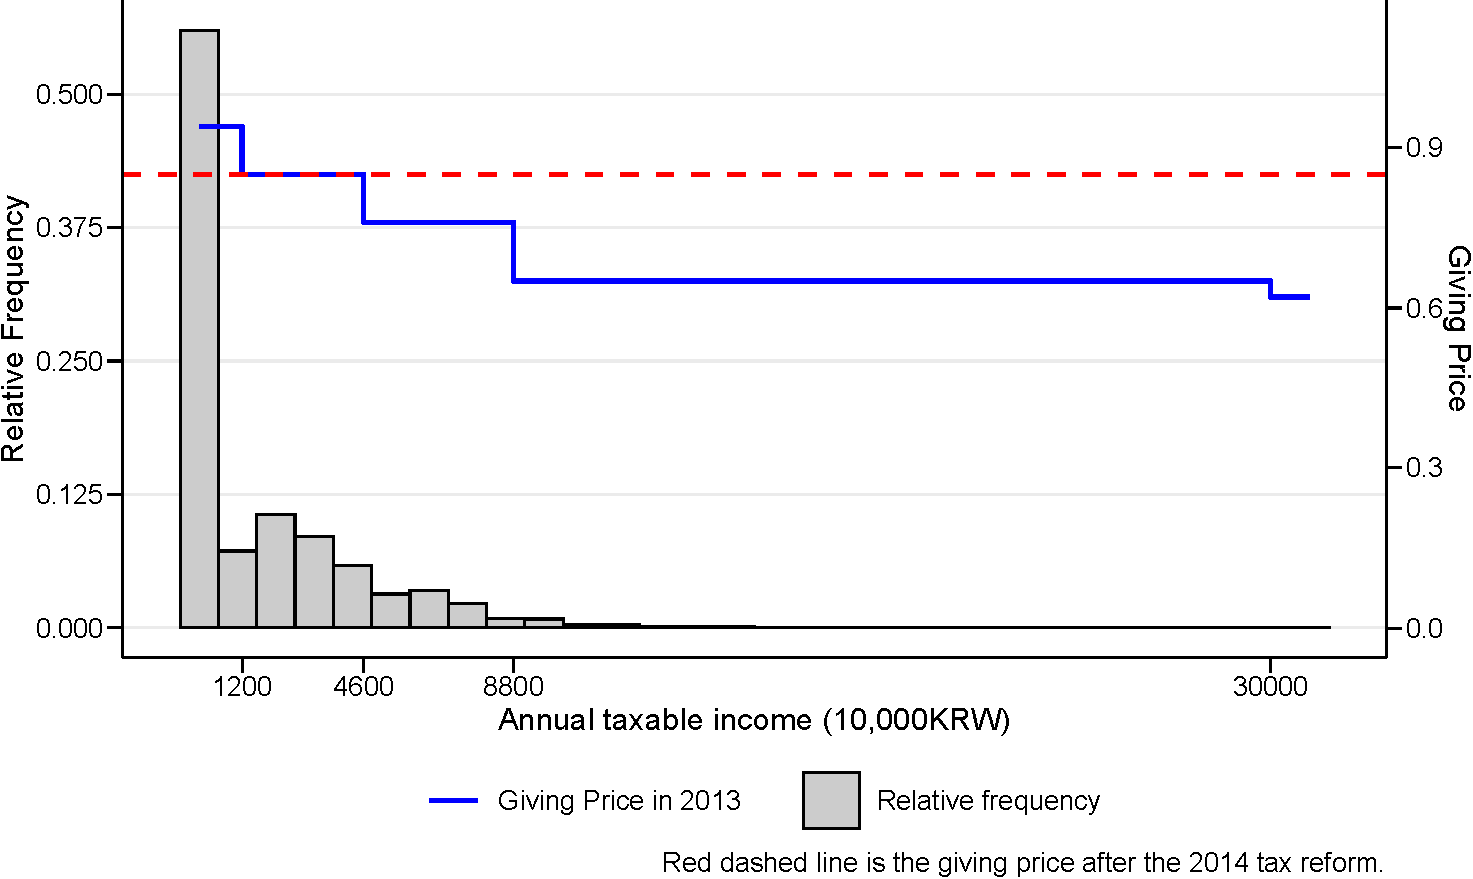
\includegraphics[width=0.7\linewidth,]{C:/Users/vge00/Desktop/NaSTaB/docs/slide/slide_files/figure-beamer/SummaryPrice-1} 

}

\caption{Income Distribution in 2013 and Relative Giving Price. Notes: The left and right axis measure the relative frequency of respondents (grey bars) and the relative giving price (solid step line and dashed line), respectively. A solid step line and a dashed horizontal line represents the giving price in 2013 and 2014, respectively.}\label{fig:SummaryPrice}
\end{figure}
\end{frame}

\begin{frame}{Identification of Price Elasticity}
\protect\hypertarget{identification-of-price-elasticity}{}
We can create three income groups based on
a change of tax incentive due to 2014 tax reform.

\begin{enumerate}
\tightlist
\item
  \(<\) 120 million KRW

  \begin{itemize}
  \tightlist
  \item
    expand tax incentive (reduce giving price)
  \end{itemize}
\item
  \([\text{120 million KRW}, \text{460 million KRW}]\)

  \begin{itemize}
  \tightlist
  \item
    tax incentive did not change
  \end{itemize}
\item
  \(>\) 460 million KRW

  \begin{itemize}
  \tightlist
  \item
    shrink tax incentive (increase giving price)
  \end{itemize}
\end{enumerate}
\end{frame}

\begin{frame}{Summary of Giving Behavior}
\protect\hypertarget{summary-of-giving-behavior}{}
\begin{figure}[t]

{\centering 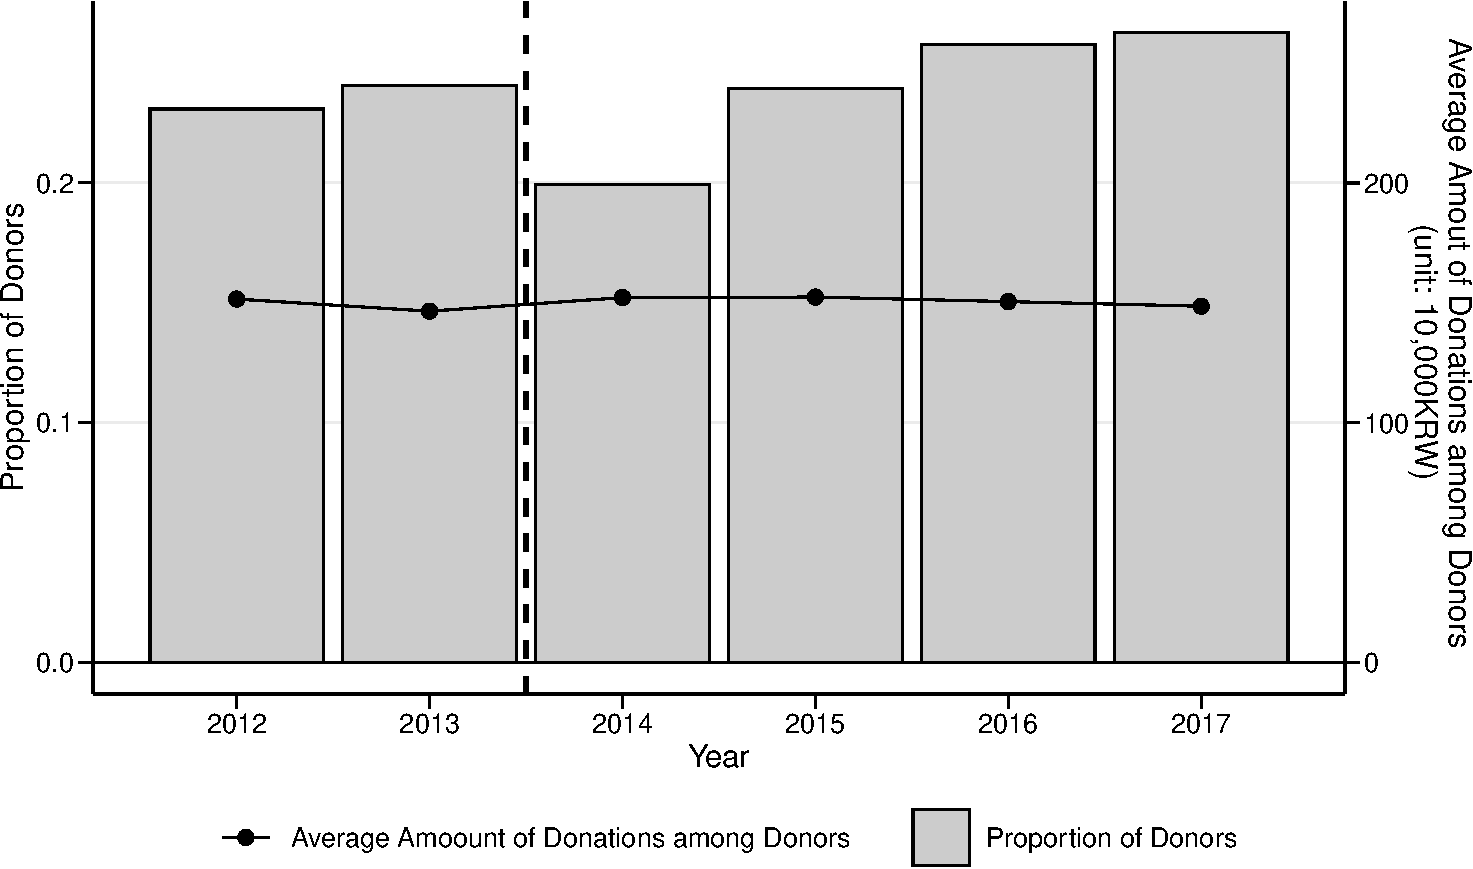
\includegraphics[width=0.7\linewidth,]{C:/Users/vge00/Desktop/NaSTaB/docs/slide/slide_files/figure-beamer/SummaryGiving-1} 

}

\caption{Proportion of Donors and Average Donations among Donors. Notes: The left and right axises measure prooortion of donors (grey bars) and the average amount of donations among donors (solid line), respectively.}\label{fig:SummaryGiving}
\end{figure}
\end{frame}

\begin{frame}{Summary of Giving Amount by Three Income Groups}
\protect\hypertarget{summary-of-giving-amount-by-three-income-groups}{}
\begin{figure}[t]

{\centering 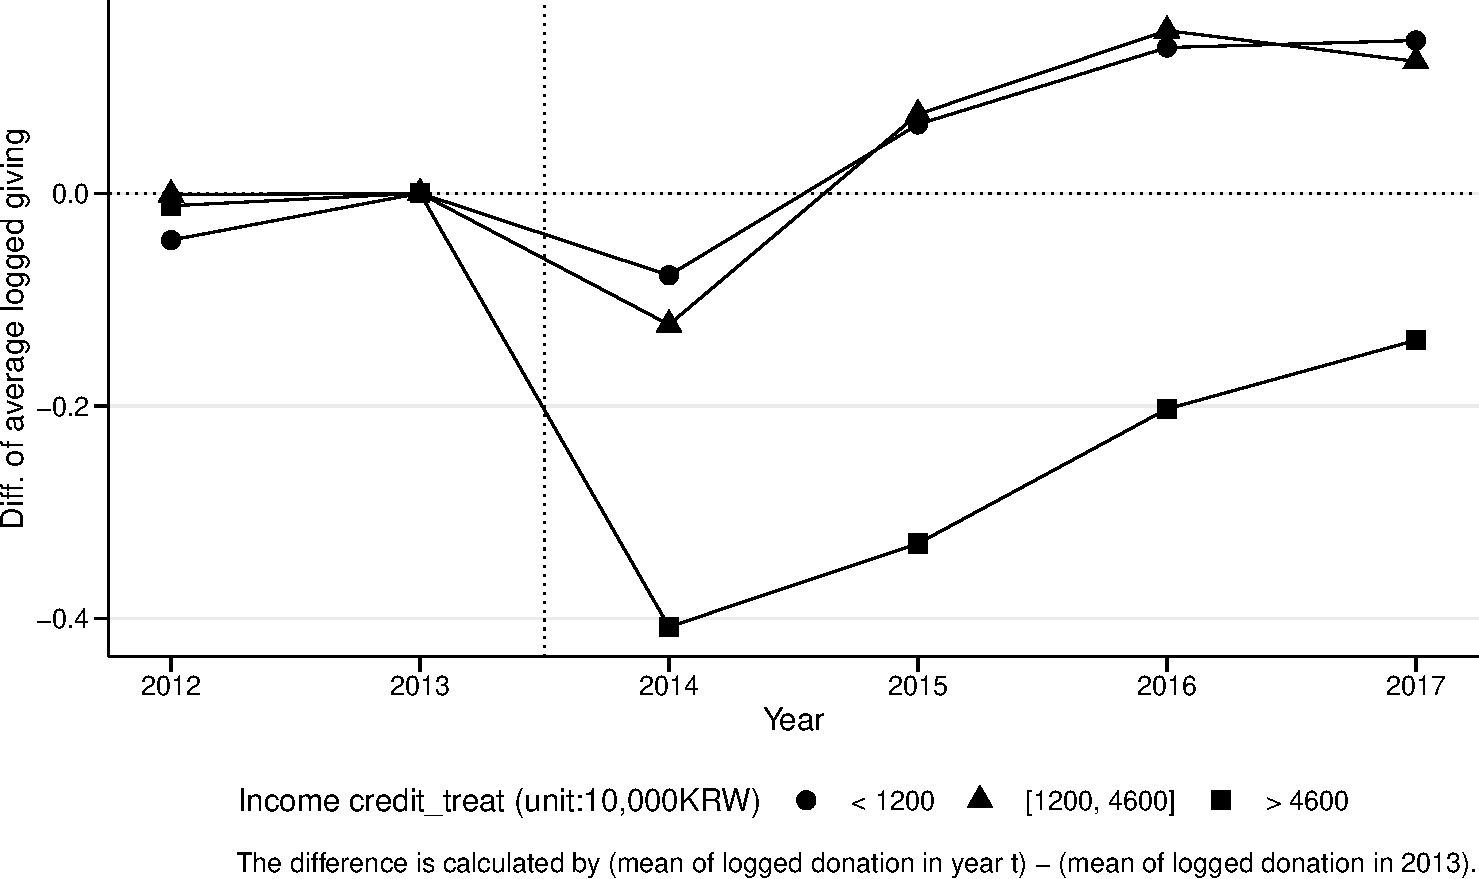
\includegraphics[width=0.7\linewidth,]{C:/Users/vge00/Desktop/NaSTaB/docs/slide/slide_files/figure-beamer/SummaryGivingOverall-1} 

}

\caption{Average Logged Giving by Three Income Groups. Notes: We created three income groups, with the relative price of giving rising (circle), unchanged (triangle), and falling (square) between 2013 and 2014. The group averages are normalized to be zero in 2013.}\label{fig:SummaryGivingOverall}
\end{figure}
\end{frame}

\begin{frame}{Summary of Giving Amount by Three Income Groups (Conditional on Donors)}
\protect\hypertarget{summary-of-giving-amount-by-three-income-groups-conditional-on-donors}{}
\begin{figure}[t]

{\centering 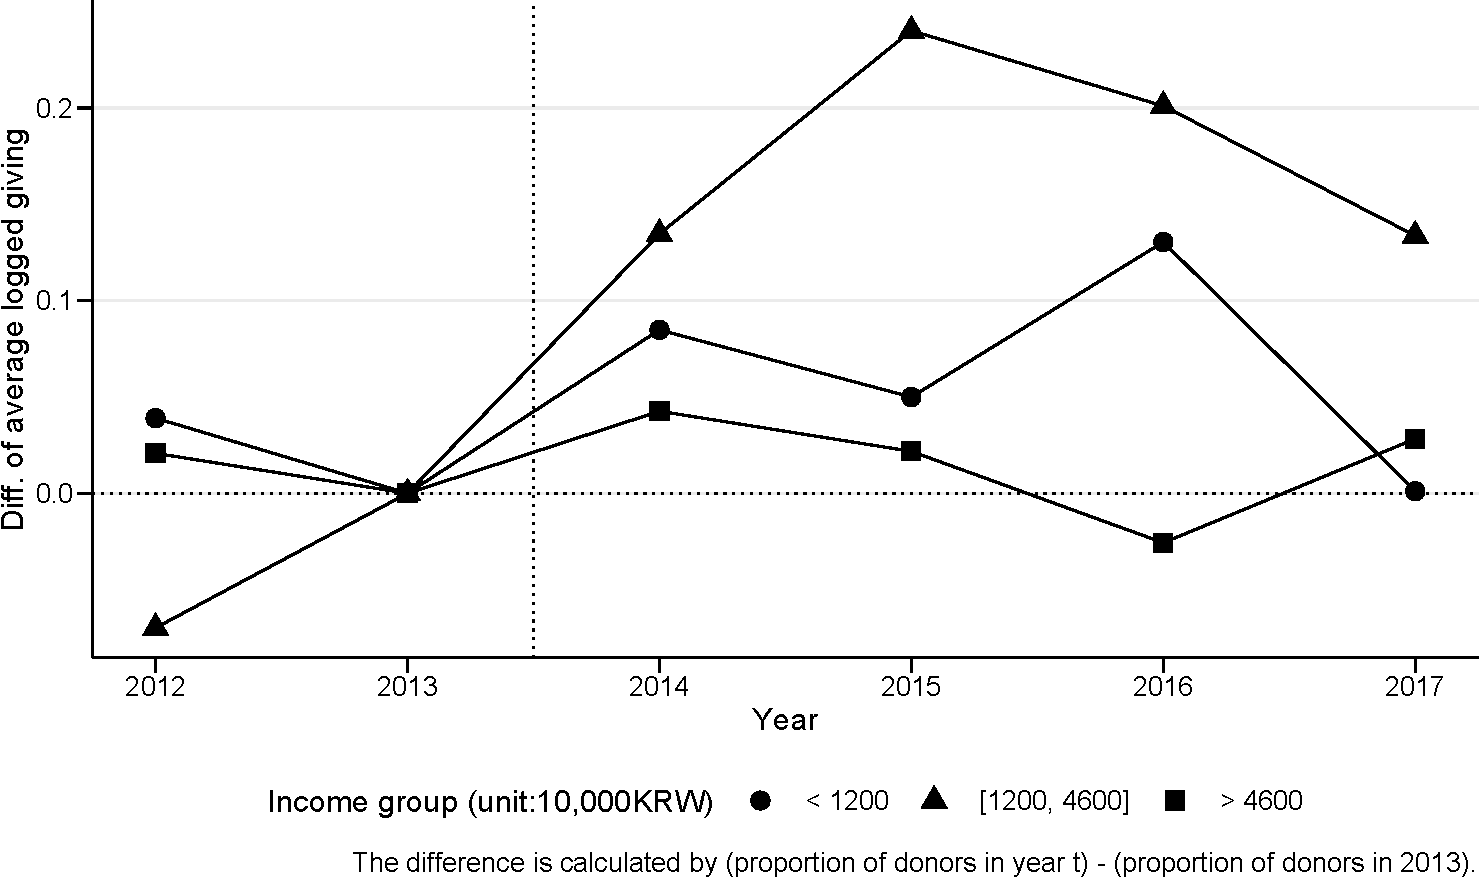
\includegraphics[width=0.7\linewidth,]{C:/Users/vge00/Desktop/NaSTaB/docs/slide/slide_files/figure-beamer/SummaryGivingIntensive-1} 

}

\caption{Average Logged Giving by Three Income Groups Conditional on Donors. Notes: We created three income groups, with the relative price of giving rising (circle), unchanged (triangle), and falling (square) between 2013 and 2014. The group averages are normalized to be zero in 2013.}\label{fig:SummaryGivingIntensive}
\end{figure}
\end{frame}

\begin{frame}{Summary of Proportion of Donors by Three Income Groups}
\protect\hypertarget{summary-of-proportion-of-donors-by-three-income-groups}{}
\begin{figure}[t]

{\centering 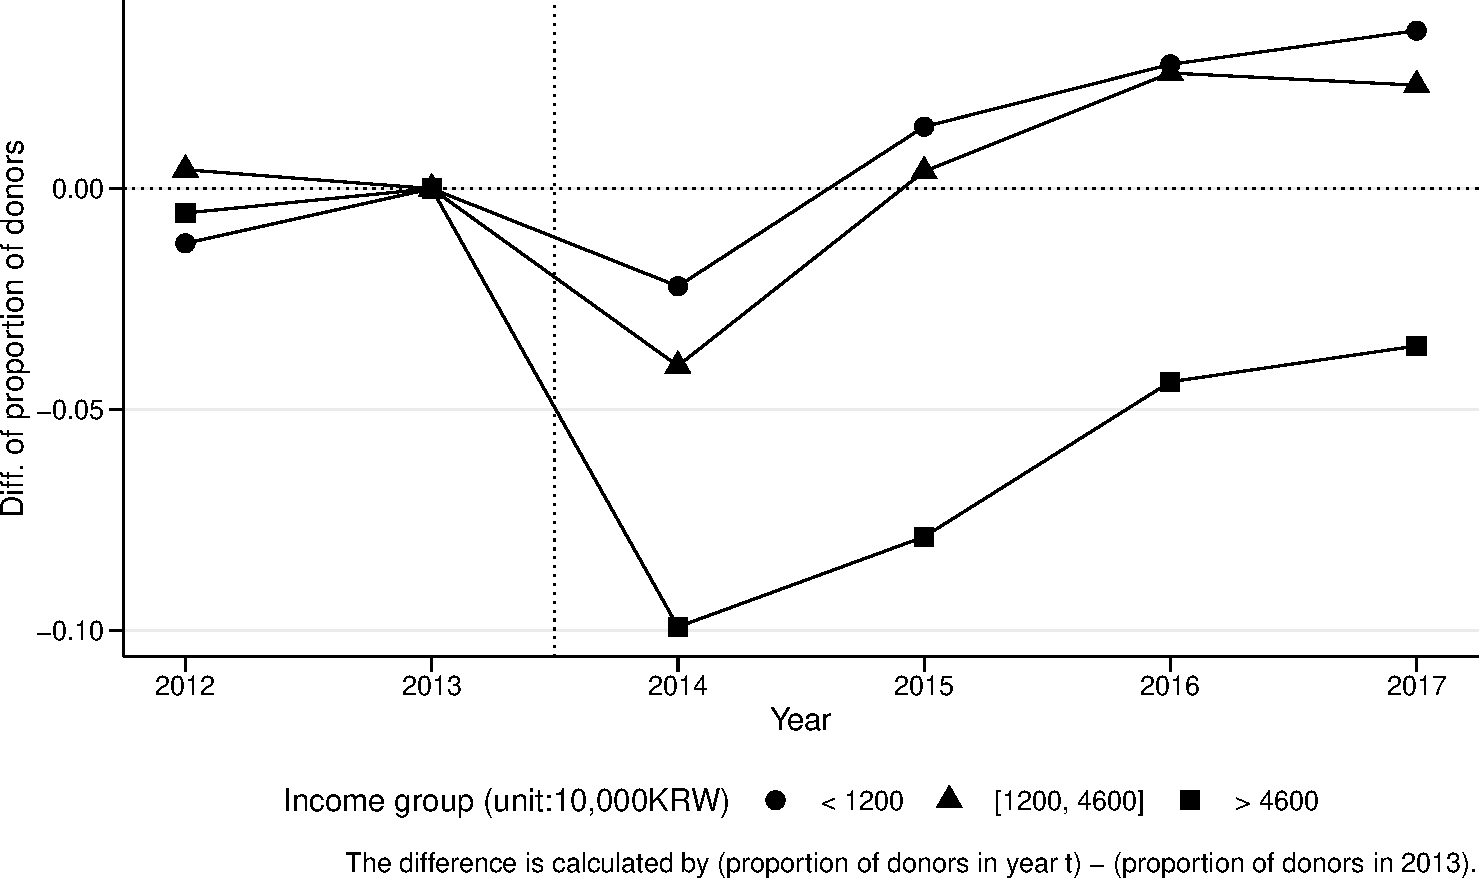
\includegraphics[width=0.7\linewidth,]{C:/Users/vge00/Desktop/NaSTaB/docs/slide/slide_files/figure-beamer/SummaryGivingExtensive-1} 

}

\caption{Proportion of Donors by Three Income Groups. Notes: We created three income groups, with the relative price of giving rising (circle), unchanged (triangle), and falling (square) between 2013 and 2014. The group averages are normalized to be zero in 2013.}\label{fig:SummaryGivingExtensive}
\end{figure}
\end{frame}

\begin{frame}{Distribution of Giving Amount by Application of Tax Relief}
\protect\hypertarget{distribution-of-giving-amount-by-application-of-tax-relief}{}
\begin{figure}[t]

{\centering 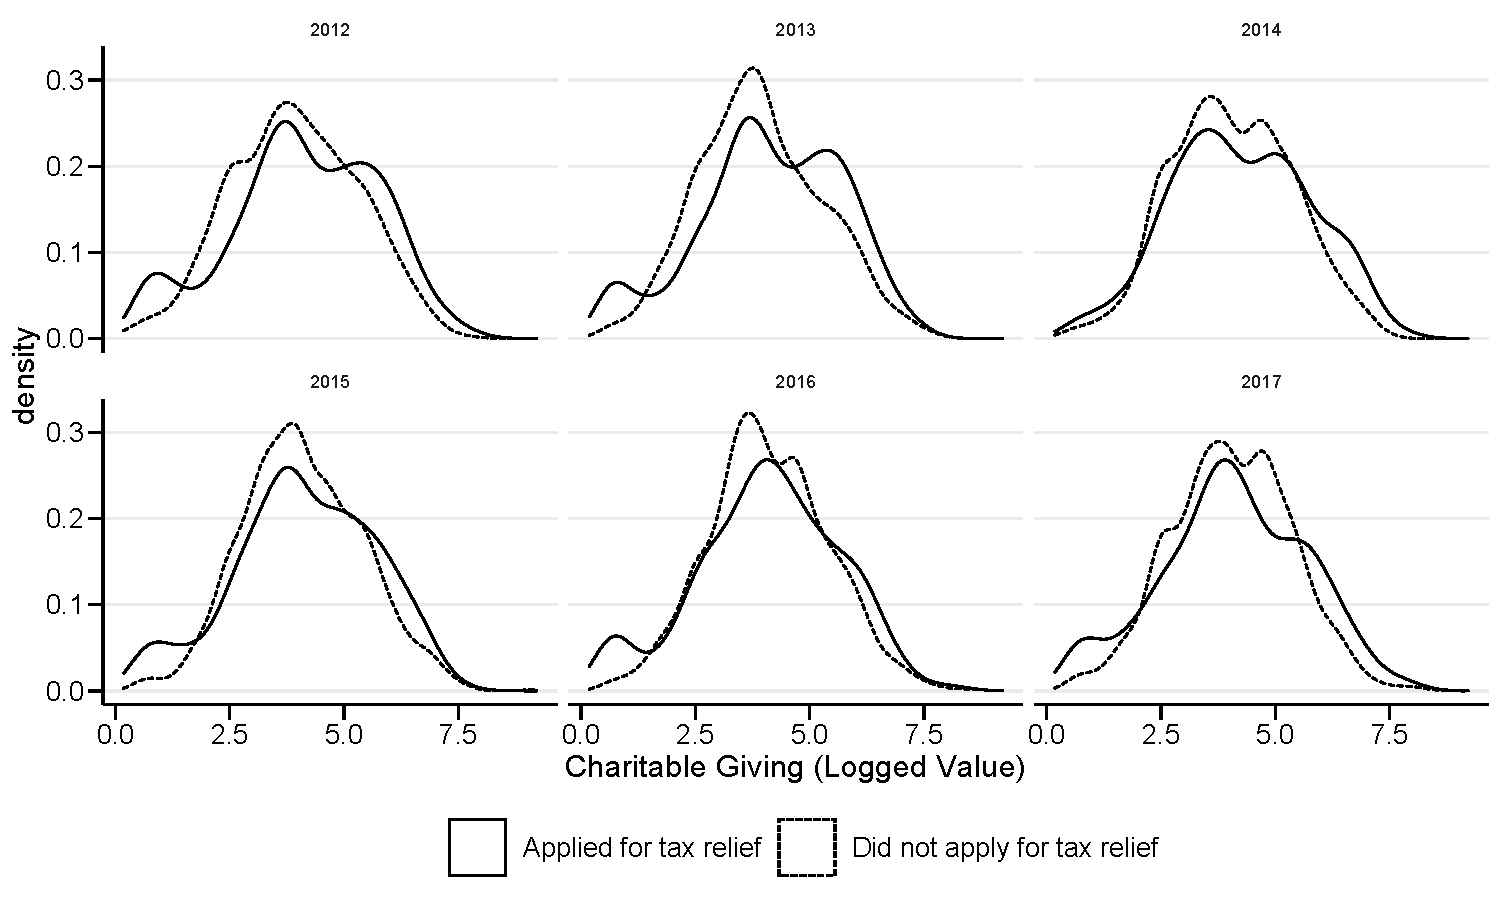
\includegraphics[width=0.7\linewidth,]{C:/Users/vge00/Desktop/NaSTaB/docs/slide/slide_files/figure-beamer/SummaryGivingIntensiveDist-1} 

}

\caption{Estimated Distribution of Charitable Giving among Donors in Each Year}\label{fig:SummaryGivingIntensiveDist}
\end{figure}
\end{frame}

\begin{frame}{Compliance Rate by Wage Earners or Not}
\protect\hypertarget{compliance-rate-by-wage-earners-or-not}{}
\begin{figure}[t]

{\centering 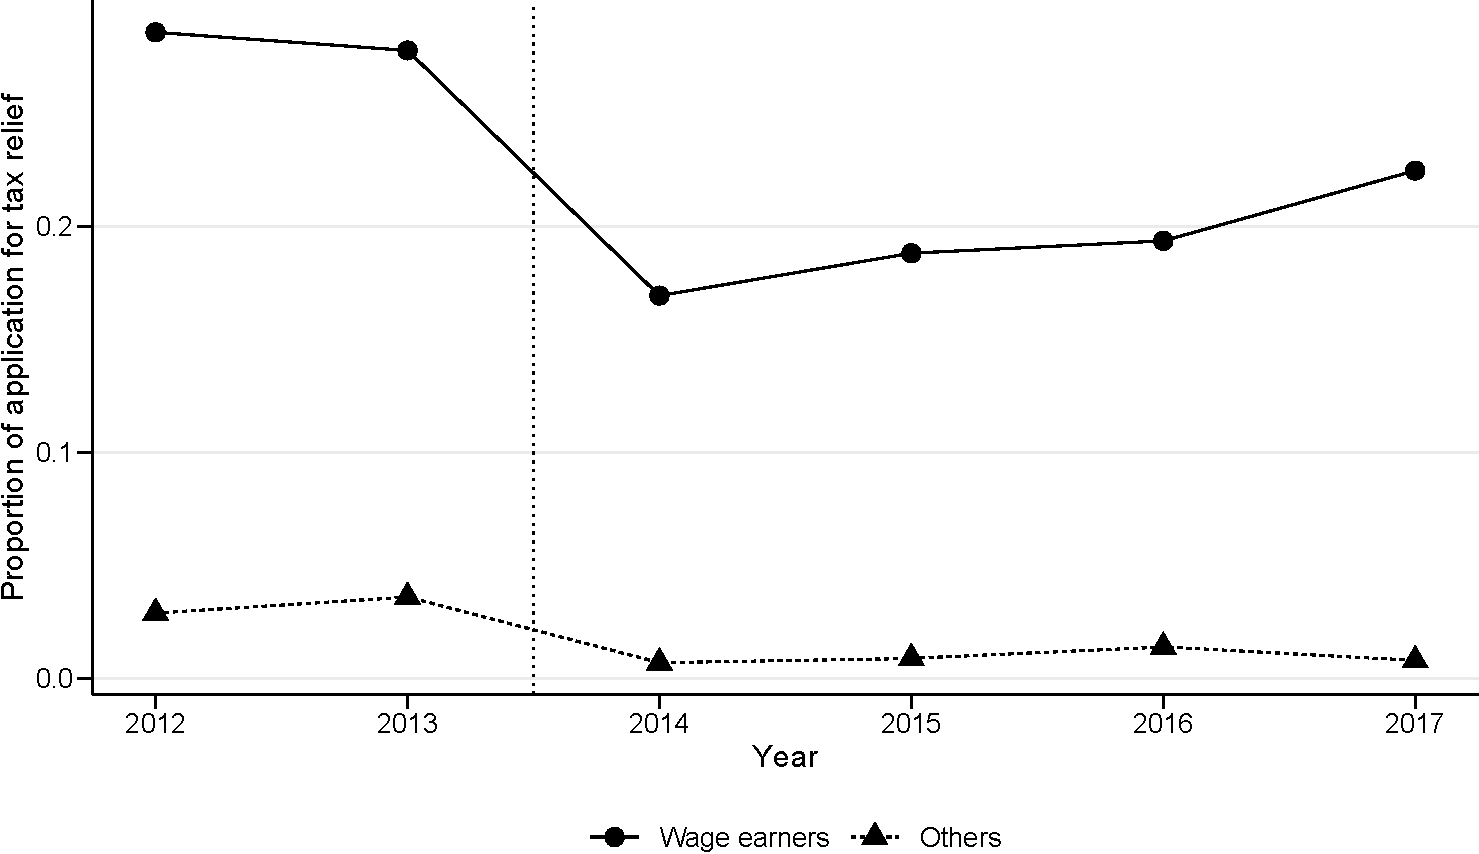
\includegraphics[width=0.7\linewidth,]{C:/Users/vge00/Desktop/NaSTaB/docs/slide/slide_files/figure-beamer/SummaryReliefbyEarner-1} 

}

\caption{Share of Tax Relief by Wage Earners. Notes: A solid line is the share of applying for tax relief among wage eaners. A dashed line is the share of applying for tax relief other than wage earners.}\label{fig:SummaryReliefbyEarner}
\end{figure}
\end{frame}

\begin{frame}{Compliance Rate by Wage Earners or Not (Conditional on Donors)}
\protect\hypertarget{compliance-rate-by-wage-earners-or-not-conditional-on-donors}{}
\begin{figure}[t]

{\centering 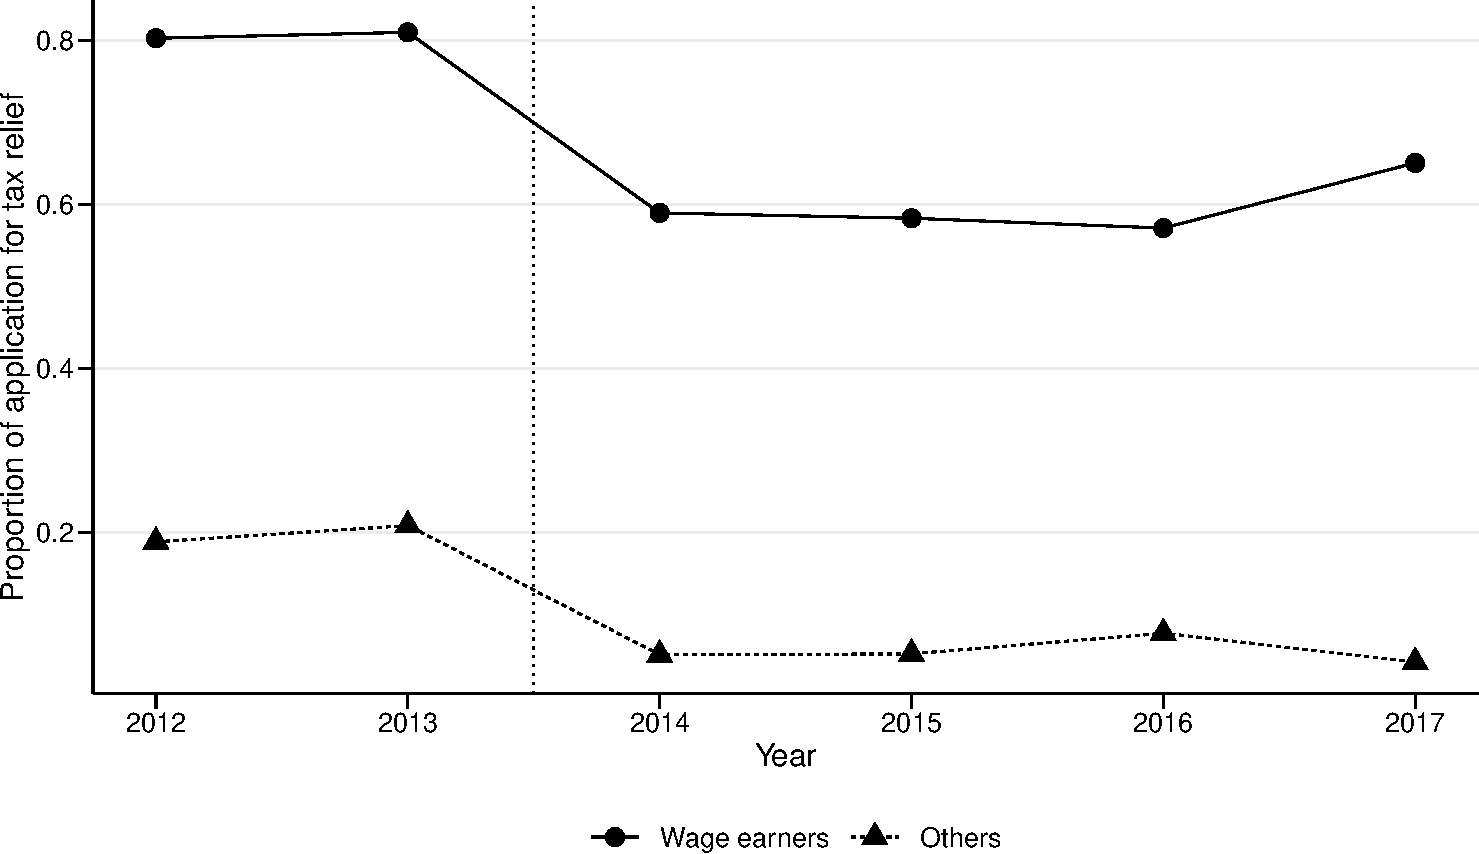
\includegraphics[width=0.7\linewidth,]{C:/Users/vge00/Desktop/NaSTaB/docs/slide/slide_files/figure-beamer/SummaryReliefbyEarner2-1} 

}

\caption{Share of Tax Relief by Wage Earners Conditional on Donors. Notes: A solid line is the share of applying for tax relief among wage eaners. A dashed line is the share of applying for tax relief other than wage earners.}\label{fig:SummaryReliefbyEarner2}
\end{figure}
\end{frame}

\hypertarget{estimation}{%
\section{Empirical Strategy}\label{estimation}}

\begin{frame}{Two Types of Price Elasticity}
\protect\hypertarget{two-types-of-price-elasticity}{}
Following Almunia et al.~(2020),

\begin{enumerate}
\tightlist
\item
  Intensive-margin price elasticity: What percentage increase in donor contributions would result from a 1\% price increase?
\item
  Extensive-margin price elasticity: What percentage increase in the donor ratio would result from a 1\% price increase?
\end{enumerate}

We use an identification strategy that combines two methods:
(1) DID using changes in tax incentives due to the 2014 tax reform and
(2) IV that captures whether or not a donation deduction is claimed due to filing costs.
\end{frame}

\begin{frame}{Intensive-Margin Price Elasticity}
\protect\hypertarget{intensive-margin-price-elasticity}{}
Two-way FE model:

\begin{align}
  \ln g_{it} = \theta_i + \gamma (R_{it} \times \ln (1 - q_{it}))
    + \beta X_{it} + \lambda_t + u_{it}, \label{eq:intensive}
\end{align}

\begin{itemize}
\tightlist
\item
  \(X_{it}\) is a vector of covariate including pre-tax income \(y_{it}\)
\item
  \(\theta_i\) and \(\lambda_t\) are individual and time FE, respectively
\item
  \(u_{it}\) is idiosyncratic error
\item
  \(\ln g_{it}\) is log-valued of amount of donations
\item
  \(R_{it}\) is a dummy of application for tax relief
\item
  \(q_{it}\) is tax incentive
\end{itemize}
\end{frame}

\begin{frame}{Extensive-Margin Price Elasticity}
\protect\hypertarget{extensive-margin-price-elasticity}{}
\begin{align}
  D_{it} = \theta_i + \delta (R_{it} \times \ln (1 - q_{it}))
    + \beta X_{it} + \lambda_t + \eta_{it}, \label{eq:extensive}
\end{align}

\begin{itemize}
\tightlist
\item
  \(D_{it}\) is a dummy indicating a donor
\item
  The parameter of interest is \(\delta\). Since the outcome variable is binary, this parameter cannot be directly interpreted as elasticity.
\item
  Extensive-margin price elasticity is obtained by \(\hat{\delta} / \bar{D}\). (\(\bar{D}\) is the sample mean of \(D_{it}\))
\end{itemize}
\end{frame}

\begin{frame}{Two Endogenous Problem}
\protect\hypertarget{two-endogenous-problem}{}
We will discuss how to resolve following two endogenous problems:

\begin{enumerate}
\tightlist
\item
  price depends on giving amount when income deduction is applied
\item
  self-selection of application for tax incentive
\end{enumerate}
\end{frame}

\begin{frame}{Endogenous Applicable Giving Price}
\protect\hypertarget{endogenous-applicable-giving-price}{}
\begin{itemize}
\item
  We use changes in tax incentives due to the 2014 tax reform as an exogenous variation of price
\item
  Endogeneity of prices cannot be completely ruled out because we use data when income deduction was applied.
\item
  The donation price when the tax relief is applied would be as follows:
  \begin{align}
  1 - q_{it} =
  \begin{cases}
    1 - T'_t(y_{it} - g_{it})  \quad\text{if}\quad t < 2014  \\
    1 - m \quad\text{if}\quad t \ge 2014
  \end{cases},
  \end{align}
\item
  Price also depends on the amount of the donation (\(g_{it}\)) during the period when the income deduction is applied.

  \begin{itemize}
  \tightlist
  \item
    This is called \emph{last}-unit price
  \end{itemize}
\end{itemize}
\end{frame}

\begin{frame}{Resolve Endogenous Applicable Giving Price}
\protect\hypertarget{resolve-endogenous-applicable-giving-price}{}
\begin{itemize}
\tightlist
\item
  Following previous studies, we use \emph{first}-unit price as an alternative to (or as IV for) last-unit price.
\item
  First-unit price is giving price with the donation amount as zero.
  \begin{align}
  1 - q^f_{it} =
  \begin{cases}
    1 - T'_t(y_{it} - 0)  \quad\text{if}\quad t < 2014  \\
    1 - m \quad\text{if}\quad t \ge 2014
  \end{cases}.
  \end{align}
\item
  the last-unit price and first-unit price coincide during the period when the tax credit is applied,
  since the donation price is independent of the donation amount.
\end{itemize}
\end{frame}

\begin{frame}{Self-Selection of Tax Incentive}
\protect\hypertarget{self-selection-of-tax-incentive}{}
\begin{itemize}
\tightlist
\item
  All donors should claim income deduction/tax credit if there is no compliance cost
  because they can obtain benefit of tax savings
\item
  Our data suggests that compliance cost is likely a major obstacle in application for tax relief.

  \begin{itemize}
  \tightlist
  \item
    24\% donor, but 10\% donors claimed income deduction/tax credit
  \item
    The distribution of donations conditional on donors does not change significantly depending on
    whether or not the tax relief is applied.
  \end{itemize}
\end{itemize}
\end{frame}

\begin{frame}{Resolve Self-Selection of Tax Incentive}
\protect\hypertarget{resolve-self-selection-of-tax-incentive}{}
\begin{itemize}
\tightlist
\item
  We exploit the fact tax system differs between wage earners and self-employed workers,
  and use a wage earner dummy (\(\text{WE}_{it}\)) as a proxy for the compliance cost.

  \begin{itemize}
  \tightlist
  \item
    Self-employed workers have to understand tax system to precisely populate tax return and retain the certificate until they submit tax return
  \item
    Wage earners need not to understand tax system and can submit the certificate at any time.
  \end{itemize}
\item
  It is necessary to assume that this variable is independent of \(u_{it}\) and \(\eta_{it}\) conditional on covariates.

  \begin{itemize}
  \tightlist
  \item
    the correlation between the salaried worker dummy and fixed effects is acceptable.
  \end{itemize}
\item
  We believe that being a salaried employee or not has no direct effect on donation behavior if we control for income and industry.
\end{itemize}
\end{frame}

\begin{frame}{Three Estimation Methods to Resolve Two Endogenous Problem (1)}
\protect\hypertarget{three-estimation-methods-to-resolve-two-endogenous-problem-1}{}
\begin{enumerate}
\tightlist
\item
  FE-2SLS with \(\text{WE}_{it} \times \ln(1 - q^f_{it})\) as an IV
\end{enumerate}

\begin{align}
  \ln g_{it} = \theta_i + \gamma (R_{it} \times \ln (1 - q^f_{it}))
    + \beta X_{it} + \lambda_t + u_{it}, \label{eq:intensive2}
\end{align}

where \(\text{WE}_{it} \times \ln(1 - q^f_{it})\) is an insturument of
\(R_{it} \times \ln (1 - q^f_{it})\)
\end{frame}

\begin{frame}{Three Estimation Methods to Resolve Two Endogenous Problem (2)}
\protect\hypertarget{three-estimation-methods-to-resolve-two-endogenous-problem-2}{}
\begin{itemize}
\item
  Remaining two methods are based on propensity socre.
\item
  Propensity score is obtained by the predicted probability of probit estimation of the following model:
  \begin{align}
  R_{it} = 1[
    \alpha_0 + \alpha_1 WE_{it} + \alpha_2 \ln(1 - q^f_{it})
    + \alpha_3 X_{it} + u_{it0} > 0
  ] \label{eq:selection}
  \end{align}
\item
  The propensity score \(\hat{P}_{it}\) is obtained by estimation using (1) full sample (pooled model)
  and (2) a subsample divided by years (separated model)

  \begin{itemize}
  \tightlist
  \item
    The former assumes coefficients are constant with rispect to year
  \item
    The latter allows coefficients to depend on year
  \end{itemize}
\end{itemize}
\end{frame}

\begin{frame}{Three Estimation Methods to Resolve Two Endogenous Problem (3)}
\protect\hypertarget{three-estimation-methods-to-resolve-two-endogenous-problem-3}{}
Again,

\begin{align*}
  \ln g_{it} = \theta_i + \gamma (R_{it} \times \ln (1 - q^f_{it}))
    + \beta X_{it} + \lambda_t + u_{it},
\end{align*}

Remaining two estimation methods:

\begin{enumerate}
\setcounter{enumi}{1}
\tightlist
\item
  We use \(\hat{P}_{it} \times \ln (1 - q^f_{it})\) as an instrument of \(R_{it} \times \ln (1 - q^f_{it})\)
\item
  We use \(\hat{P}_{it} \times \ln (1 - q^f_{it})\) instead of \(R_{it} \times \ln (1 - q^f_{it})\) as the explanatory variable.
\end{enumerate}
\end{frame}

\hypertarget{result}{%
\section{Estimation Results}\label{result}}

\begin{frame}{Main Results: Intensive-Margin Price Elasticity}
\protect\hypertarget{main-results-intensive-margin-price-elasticity}{}
\begin{table}
\centering
\fontsize{8}{10}\selectfont
\begin{threeparttable}
\begin{tabular}[t]{>{\raggedright\arraybackslash}p{10em}cccccc}
\toprule
\multicolumn{1}{c}{ } & \multicolumn{3}{c}{FE} & \multicolumn{3}{c}{FE-2SLS} \\
\cmidrule(l{3pt}r{3pt}){2-4} \cmidrule(l{3pt}r{3pt}){5-7}
  & (1) & (2) & (3) & (4) & (5) & (6)\\
\midrule
Applying tax relief x log(first price) & \num{-0.748}*** &  &  & \num{-1.400}*** & \num{-1.437}*** & \num{-1.540}***\\
 & (\num{0.225}) &  &  & (\num{0.411}) & (\num{0.363}) & (\num{0.375})\\
PS of applying tax relief x log(first price) &  & \num{-1.544}*** & \num{-1.515}*** &  &  & \\
 &  & (\num{0.388}) & (\num{0.367}) &  &  & \\
log(income) & \num{1.408} & \num{0.833} & \num{0.824} & \num{0.937} & \num{0.909} & \num{0.830}\\
 & (\num{1.113}) & (\num{1.121}) & (\num{1.121}) & (\num{1.119}) & (\num{1.098}) & (\num{1.094})\\
\midrule
First-stage: Instrument &  &  &  & 0.638 & 1.075 & 0.984\\
 &  &  &  & {}[468.1] & {}[534.6] & {}[662.2]\\
Num.Obs. & \num{7004} & \num{6975} & \num{6975} & \num{6975} & \num{6975} & \num{6975}\\
Instrument &  &  &  & WE x Price & PS x Price & PS x Price\\
Method of PS &  & Pool & Separate &  & Pool & Separate\\
\bottomrule
\end{tabular}
\begin{tablenotes}
\item Notes: $^{*}$ $p < 0.1$, $^{**}$ $p < 0.05$, $^{***}$ $p < 0.01$. Standard errors are clustered at individual level. A square bracket is wald statistics of instrument.
\end{tablenotes}
\end{threeparttable}
\end{table}
\end{frame}

\begin{frame}{Main Results: Extensive-Margin Price Elasticity}
\protect\hypertarget{main-results-extensive-margin-price-elasticity}{}
\begin{table}
\centering
\fontsize{8}{10}\selectfont
\begin{threeparttable}
\begin{tabular}[t]{>{\raggedright\arraybackslash}p{10em}cccccc}
\toprule
\multicolumn{1}{c}{ } & \multicolumn{3}{c}{FE} & \multicolumn{3}{c}{FE-2SLS} \\
\cmidrule(l{3pt}r{3pt}){2-4} \cmidrule(l{3pt}r{3pt}){5-7}
  & (1) & (2) & (3) & (4) & (5) & (6)\\
\midrule
Applying tax relief x log(first price) & \num{-2.800}*** &  &  & \num{-0.464}*** & \num{-0.563}*** & \num{-0.738}***\\
 & (\num{0.074}) &  &  & (\num{0.176}) & (\num{0.120}) & (\num{0.116})\\
PS of applying tax relief x log(first price) &  & \num{-0.452}*** & \num{-0.566}*** &  &  & \\
 &  & (\num{0.107}) & (\num{0.101}) &  &  & \\
log(income) & \num{0.975}*** & \num{1.950}*** & \num{1.844}*** & \num{2.121}*** & \num{2.072}*** & \num{1.986}***\\
 & (\num{0.233}) & (\num{0.279}) & (\num{0.278}) & (\num{0.279}) & (\num{0.261}) & (\num{0.256})\\
\midrule
Implied price elasticity & -10.799*** & -1.741*** & -2.181*** & -1.788*** & -2.169*** & -2.841***\\
 & (0.287) & (0.411) & (0.388) & (0.678) & (0.463) & (0.448)\\
First-stage: Instrument &  &  &  & 0.289 & 0.803 & 0.768\\
 &  &  &  & {}[276.6] & {}[311.7] & {}[361.9]\\
Num.Obs. & \num{27017} & \num{26863} & \num{26863} & \num{26863} & \num{26863} & \num{26863}\\
Instrument &  &  &  & WE x Price & PS x Price & PS x Price\\
Method of PS &  & Pool & Separate &  & Pool & Separate\\
\bottomrule
\end{tabular}
\begin{tablenotes}
\item Notes: $^{*}$ $p < 0.1$, $^{**}$ $p < 0.05$, $^{***}$ $p < 0.01$. Standard errors are clustered at individual level. A square bracket is wald statistics of instrument.
\end{tablenotes}
\end{threeparttable}
\end{table}
\end{frame}

\begin{frame}{Robustness Check}
\protect\hypertarget{robustness-check}{}
\begin{itemize}
\tightlist
\item
  \emph{Exclude Annoucement Effect}

  \begin{itemize}
  \tightlist
  \item
    intertemporal substitution due to annoucement of 2014 tax reform
  \item
    We drop observations in 2013 and 2014
  \item
    Estimated elasticity does not change significantly
  \end{itemize}
\item
  \emph{Last-unit Price Elasticity}

  \begin{itemize}
  \tightlist
  \item
    The acutual price that decision-makers face is \emph{last-unit}
    (especially, intensive-margin decision)
  \item
    We use first-unit price as an instrument of last-unit one
  \item
    Last-unit price elasticity is more elastic
    than first-unit price elasticity
  \end{itemize}
\end{itemize}
\end{frame}

\end{document}
